\documentclass[11pt]{exam}

\usepackage{amsmath}
\usepackage{graphicx}
\usepackage{geometry}
\usepackage{etoolbox}
\BeforeBeginEnvironment{choices}{\par\nopagebreak\minipage{\linewidth}}
\AfterEndEnvironment{choices}{\endminipage}
\geometry{
a4paper,
total={185mm,257mm},
left=10mm,
top=25mm,
bottom=10mm
}

\begin{document}
\setlength{\voffset}{-0.5in}
\setlength{\headsep}{5pt}

\fbox{\fbox{\parbox{8cm}{\centering
\vspace{2mm}
Testat - Versuch J - Ultraschall 
\vspace{2mm}
}}}
\hspace{2mm}
\makebox[0.25\textwidth]{Name:\enspace\hrulefill} \hspace{5mm}
\makebox[0.2\textwidth]{Datum:\enspace\hrulefill}
\vspace{4mm}

\begin{questions}

\question In der Graphik (beliebige Einheiten) wird die Periodendauer wiedergegeben durch ... ? 

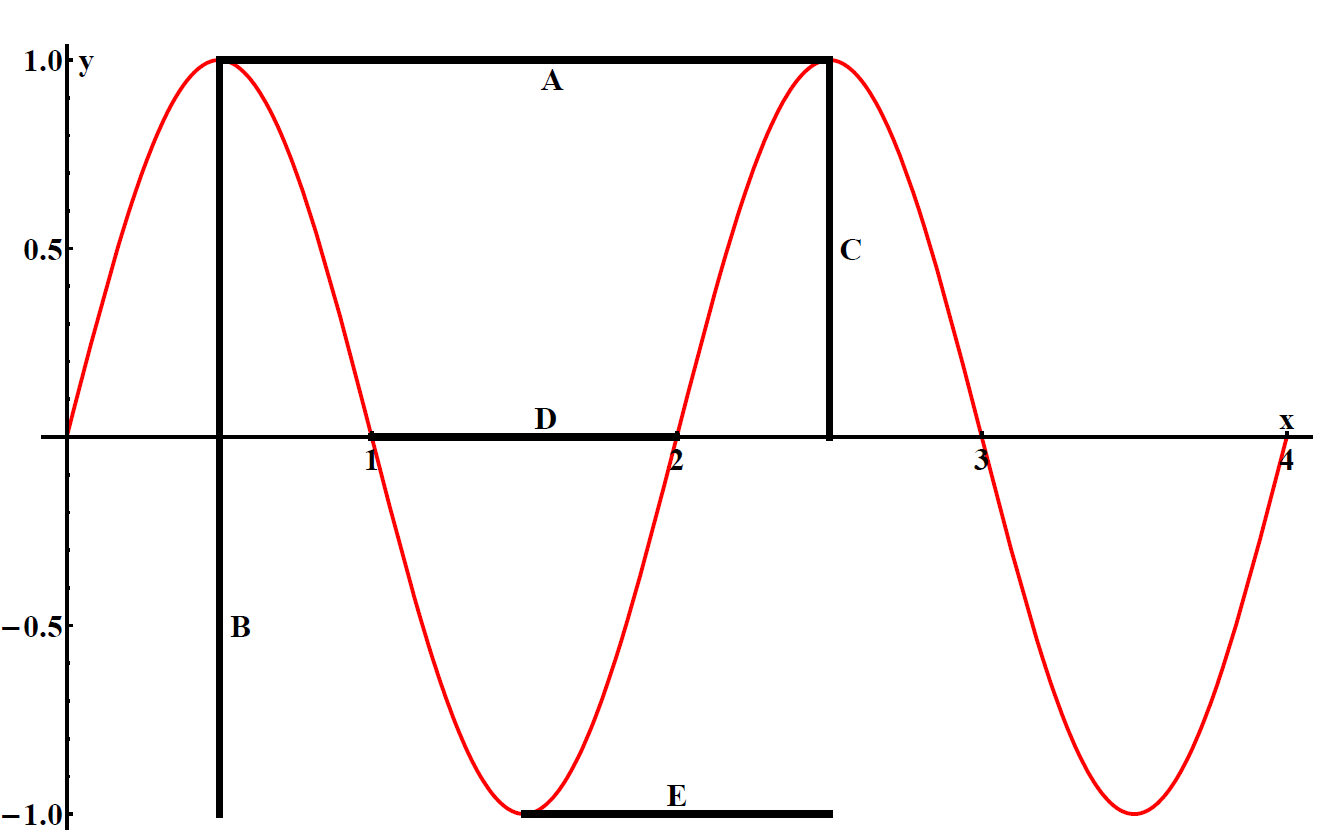
\includegraphics[width=0.4\textwidth]{images/Sinuskurve.png}

\begin{choices}
	\choice Linie B
	\choice Linie C
	\choice Linie D
	\choice Linie E
	\choice Linie A (correct)
\end{choices}

\vspace{3mm}\question Wie groß ist die Schallgeschwindigkeit in Luft bei Normalbedingungen?

\begin{choices}
	\choice \( \mathrm{3,43~\frac{m}{s}} \)
	\choice \( \mathrm{343~\frac{mm}{s}} \)
	\choice \( \mathrm{0,343~\frac{km}{s}} \) (correct)
	\choice \( \mathrm{34,3~\frac{cm}{s}} \)
	\choice \( \mathrm{343~\frac{km}{h}} \)
\end{choices}

\vspace{3mm}\question Welche Frequenz \( f \) hat eine Schallwelle in Luft mit der Periodendauer \( T= \mathrm{10~s} \) ?

\begin{choices}
	\choice 100 Hz
	\choice 3430 Hz
	\choice 10 Hz
	\choice 0,1 Hz (correct)
	\choice 343 Hz
\end{choices}

\vspace{3mm}\question In welchem Bereich liegen die für den Menschen hörbaren Frequenzen?

\begin{choices}
	\choice 20 Hz bis 200 Hz
	\choice 2 kHz bis 200 kHz
	\choice 20 kHz bis 2 kHz
	\choice 20 kHz bis 20 MHz
	\choice 20 Hz bis 20 kHz (correct)
\end{choices}

\vspace{3mm}\question Welche Aussagen zur Schallerzeugung und -ausbreitung sind zutreffend?	* Schallwellen können mit einem Piezo-Kristall erzeugt werden.	* Schallwellen können durch schwingende Membranen erzeugt werden.	* Die Schallgeschwindigkeit ist in Vakuum höher als in Luft, da die Schallwellen nicht durch Luftmoleküle gebremst werden.	* In Festkörpern ist die Schallgeschwindigkeit kleiner als in Luft, da die Moleküle nicht so schnell ausgelenkt werden können. 

\begin{choices}
	\choice Nur Ausage 1 und 3 sind richtig.
	\choice Nur Ausage 1 und 2 sind richtig. (correct)
	\choice Nur Ausage 2 und 4 sind richtig.
	\choice Nur Ausage 2 und 3 sind richtig.
	\choice Nur Ausage 3 und 4 sind richtig.
\end{choices}

\vspace{3mm}\end{questions}

\end{document}
